%% The following is a directive for TeXShop to indicate the main file
%%!TEX root = diss.tex

\chapter{Introduction}
\label{ch:introduction}
Technology changes.
Symbolic, machine-focused communication like punch cards, assembly languages, and terminal interfaces yield to natural, physical, always-connected interactive systems.
The emergence of virtual and augmented reality (VR \& AR), rapid development of personal fabrication techniques, and explosion of wearable and cyberphysical technologies propel us towards a mixed physical-digital world at an accelerating pace.
%As computers expand beyond screens and speakers, we look not just to vision and sound, but also the rich senses of touch.
As computers expand beyond screens and keyboards, we look to engage the rich senses of touch.



%Human beings are physical, social creatures, yet our technology has only just started to communicate on our terms.
%Over the years, computing has progressed from symbolic, machine-focused communication like punch cards, assembly languages, and terminal interfaces to physical and natural user interaction.
%Despite embracing new interaction techniques like touchscreens and voice control, the rich senses of touch have been relegated to buzzing alerts or limited to high-stakes expert systems like laparoscopic surgery.

Haptic experiences are moving from niche roles to mainstream adoption.
Haptic technology includes both the tactile (skin-based) and proprioceptive (force- and position-based) components of touch.
Recently, other natural interaction techniques like touchscreens and voice control held the limelight, with haptic feedback relegated to buzzing alerts or limited to high-stakes expert systems like laparoscopic surgery.
Now, new media seeks deeper immersion, smart environments look to connect physically with users, and consumer devices like the Apple Watch and Pebble adopt high-fidelity haptic actuators.
The question is how to enable designers to craft experiences with these technologies.

The diverse field of haptics has seen active engineering of new devices and study of human perception, but the design of haptic experiences remains a critical challenge.
Little is known about this nascent field of design, with many unique challenges: real-world haptic experiences are rich, diverse, multimodal entities which necessitate in-person interaction, while synthesized haptics strive to be.
How can we support creativity with these experiences, empowering artists, developers, designers, and scientists to effectively work with this emerging medium?
In this dissertation, we study the process of haptic experience design (\haxd) and establish guidelines for building interactive software systems to support it.
%Through a series of implemented tools, we build pathways for haptic designers.
%This is complemented by both quantitative and qualitative inquiry to understand how haptic designers' experiences and their process.
%Critically, we examine contextual activities that are naturally supported in non-haptic design design, but break down when applied to touch-based interactions: sketching, editing, browsing, and sharing.
%
%
%\section{The state of haptic experience design}
%Haptics is great for many applications.
%Some of the highest profile benefits come from high-resolution medical contexts like remote surgery or dentistry simulation.
%More prevalent, wearables have opened up a wide variety of contexts for unobtrusive tactile feedback, such as exercise bands.
%Accessibility remains an important use for touch-based technology for when other modalities are unavailable.
%Affective display, like communicating the emotions of a loved one, can take advantage of the personal nature of touch.
%%VR \& AR
%
%Of course, lots of work has gone into understanding how to make effective haptics.
%Design guidelines tell us effective ways to communicate large sets of information, provide spatial guidance, and even how to perform tactile concerts.
%% tactile icons and tactons to more sophisticated affective qualities ...
%Several editors and design tools have been built to create
%However, they don't consider the wider context of design: the fact that creativity is a social process that takes place in our environment, where designers build upon new ideas, receive feedback from others, and incroporate their personal experience into their designs.
%
%
%
%
%\section{Creativity in context}
%A painter snatches her paintbrush, sets her easel, and begins.
%An image of \emph{La Grande Jatte} slowly emerges, one stroke at a time, each colour carefully considered.
%What is missing from this scene?
%First, the landscape: is it laid out in front of our painter, referenced from a photograph, remembered, or purely imagined?
%Does she stand alone, or is there a friend giving an impression?
%How does she feel on this particular day, and is she painting for fun or money (or both)?
%
%In this dissertation, I make a simple argument: context must be considered for creative tasks. I then apply this argument to haptic experience design.
%The central goal is arguing for an embodied process of design, a systems model of design. This is applied to both a single haptic experience (consider hardware, user, etc. and all the challenges that this system entails), and to the designer?s process, situated in customers, colleagues, examples, and the design right in front of her.
%
%Many people have argued that creativity is not a solitary endeavor; Mihaly (cite), Warr (cite), shneiderman (...). Buxton, ... .
%Recent design research has empirically evaluated this ... Kellmmer, Dow, Hartmann, ... .
%
%Ultimately, creativie interfaces must have low-bar, wide walls, high ceiling; haptic desogn has none of these.
%
%
%
%\section{The difference of haptics}
%By applying advanced design and creativity thinking to haptics, we find two things: 
%1) a way to further improve haptic design, empowering designers, developers, and end-users to create for this new field, and 
%2) a confirmation and elaboration on design thinking.
%Many ideas that are taken for granted in graphic design break down when applied to haptics. 
%This makes us think more critically about design and creativity, and can inform other fields by showing us how haptic experience design is different, and supporting design processes for other, future technologies that are still emerging. (Examples ???)
%
%
%\section{Approach and Contributions}
%describe methodology - design working tools, study process, design extra toools, design haptics, and talk to designers from ground up.
%Multi-pronged approach to understanding this problem.
%
%List of chapters here:
%
%
%
%\osC{bookmark}
%Haptic sensations enable engaging, personal, and low-attention experiences, but this is limited due to little support for \emph{designing} a haptic sensation.
%Computer-controlled haptic experiences are a recent phenomenon; the focus on technology requirements and rapidly changing field has left little room for examining processes of design in a methodical way.
%


\section{Haptic Experience Design (HaXD)}
We define \haxd\ as: % ``haptic experience design'' (\haxd) as:
\begin{quote}
\it The design (planning, development, and evaluation) of user experiences  deliberately connecting interactive technology to
% intentionally involving both interactive technology and
one or more perceived senses of touch, possibly as part of a multimodal or multisensory experience.\footnote{We developed this definition from our interviews with hapticians (\autoref{ch:hapticianinterviews}).}
\end{quote}
We use \haxd instead of ``haptic design", which can also refer to design practices related to haptics but not directly involving the user experience, \eg, mechanical design of a new display mechanism. % or software design of a new control method.
%Our definition also includes pseudo-haptics \cite{Pusch2011} and other illusions that trick the user into thinking haptic feedback is occurring without direct tactile or kinesthetic stimulation.
%OS 06.09 should we also include tangibles?
We use ``haptic designers" or ``hapticians" to refer to haptic \emph{experience} designers (those who practice \haxd).
%In this work, we shed light on \haxd, documenting the challenges that are unique to or accentuated in haptic design, and applying  design thinking to those challenges.

In this dissertation, we take a systems approach to design.
Designers do not exist in a vacuum, but rather in in a physical, personal, social, and cultural context. %, and are shaped by their personal experiences.
We adopt a framework of design activities which are practiced in general experience design, but need explicit support in \haxd.
Our research identified four activities (\autoref{fig:intro:buxtonaugmented}): \emph{sketching}, ad-hoc, suggestive exploration; \emph{refining}, iteration and fine-tuning; \emph{browsing} examples and drawing from experience; and \emph{sharing} designs for feedback and posterity.
Chapters \ref{ch:hapticinstrument}-\ref{ch:hapturk} explore these activities directly. %, which were identified through those projects.





\begin{figure}[htbp] %  figure placement: here, top, bottom, or page
   \centering
   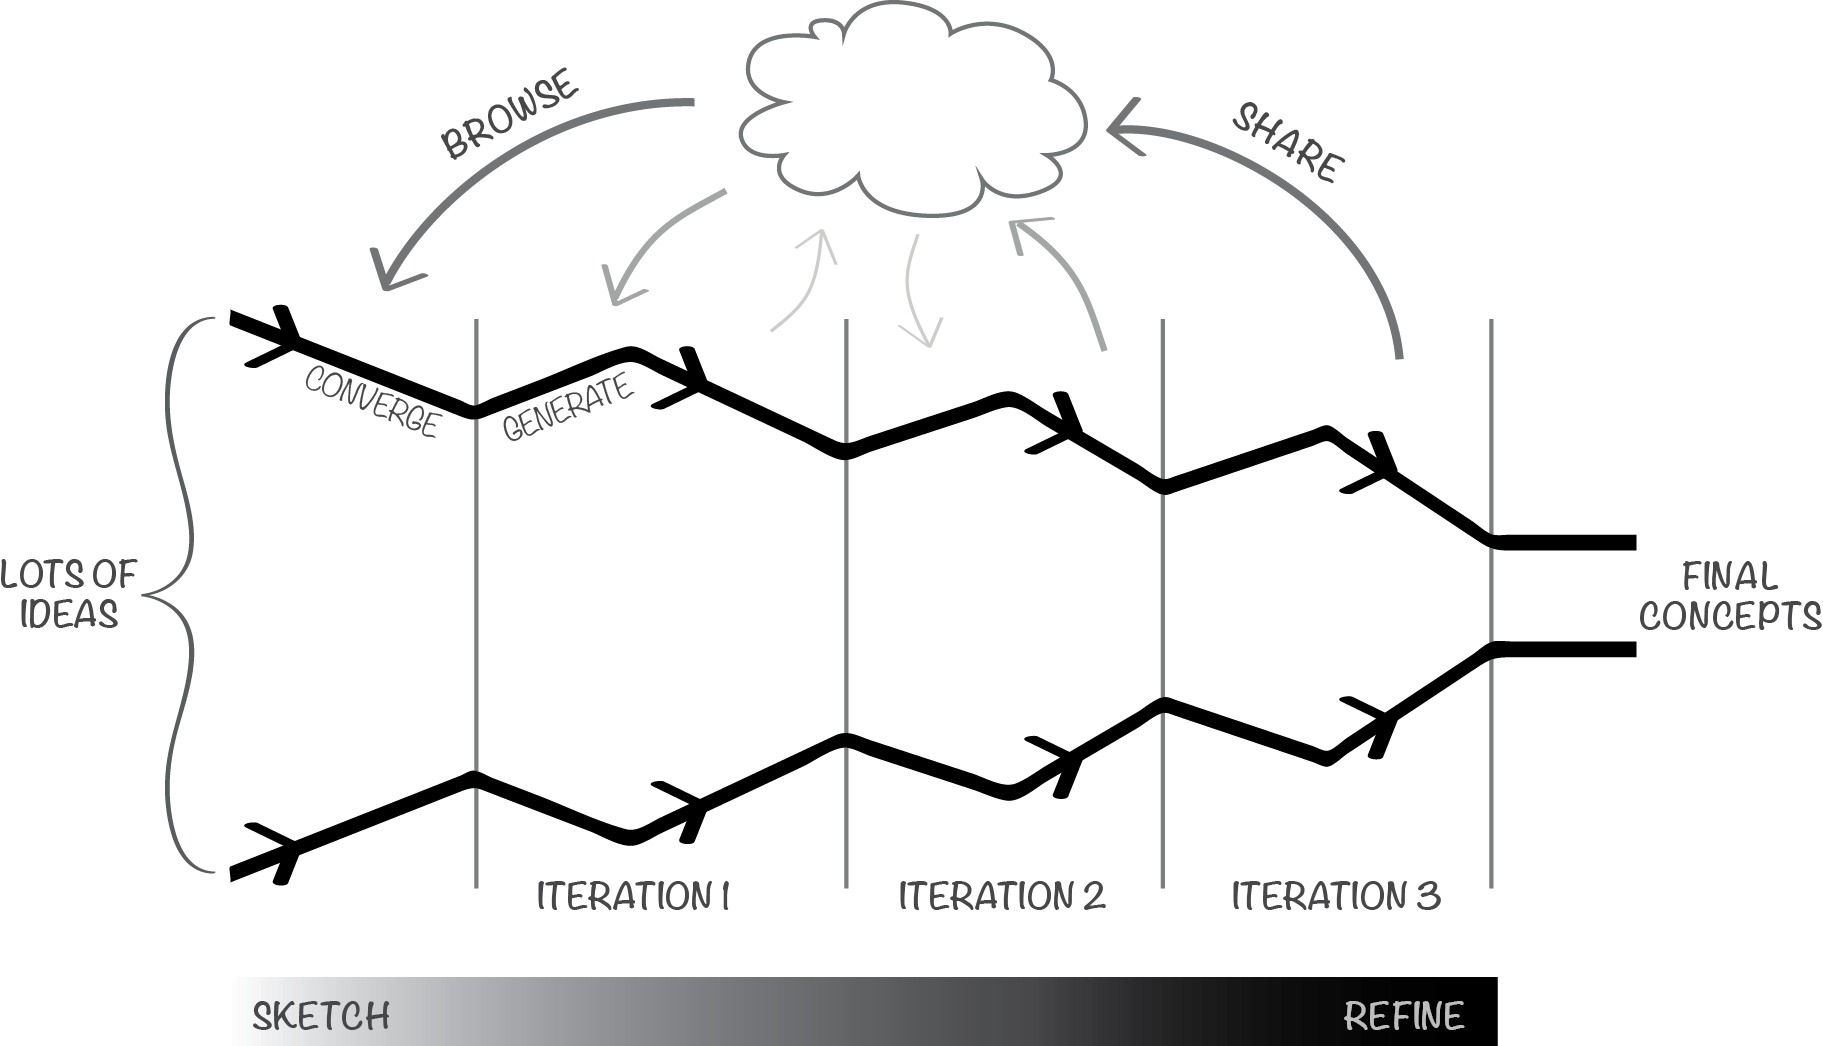
\includegraphics[width=\textwidth,height=2.6in]{Fig1-4_Buxton-Adapted} 
   \caption{The classic design funnel, adapted from \citet{Buxton2007}.
   Multiple initial ideas are iteratively developed into final concepts.
   We add four design activities that occur across design fields, but need to be explicitly supported for \haxd: \textit{sketching}, \textit{refining}, \textit{browsing}, and \textit{sharing}.}
   \label{fig:intro:buxtonaugmented}
\end{figure}





\section{Why is \haxd hard?}
Two major types of challenges facing \haxd are those resulting from its relative youth, and those intrinsic to the sense of touch and touch-based technology.
One goal of this dissertation is to articulate the challenges that have been known informally for years, and capture those that are not as well known.

The first conference to explicitly focus on haptics was the Haptics Symposium in 1992, which focused on engineering concerns.
As a result, design for haptic experiences is not as mature as with vision and audio, which can draw from centuries of music and graphic design, and decades of sound design, and translate well to their digital equivalents.
We see this in the limited infrastructure to support the wide variety of haptic devices \cite{Hayward2007}, to the point where online distribution is current research \cite{AbdurRahman2010}, and with limited, varied language for touch \cite{Jansson-Boyd2011}.

There are also intrinsic challenges when designing for touch:
variabilities in low-level perception due to, \eg, individual differences \cite{Lo1984}, device location and user activity \cite{Karuei2011}, and aging \cite{Stevens1996,Stevens1992};
a strong influence of user preferences \cite{Seifi2014,Seifi2015};
complexity of the haptic senses \cite{ChoiKuchenbecker2013,Lederman2009survey,Kandel2000};
and tight technical constraints cross-cutting software and hardware \cite{levitin2000perception,Hayward2007}.
Throughout this work, we identify and characterize these challenges, and make progress to conquer them.




\begin{figure}[htbp]
\begin{center}
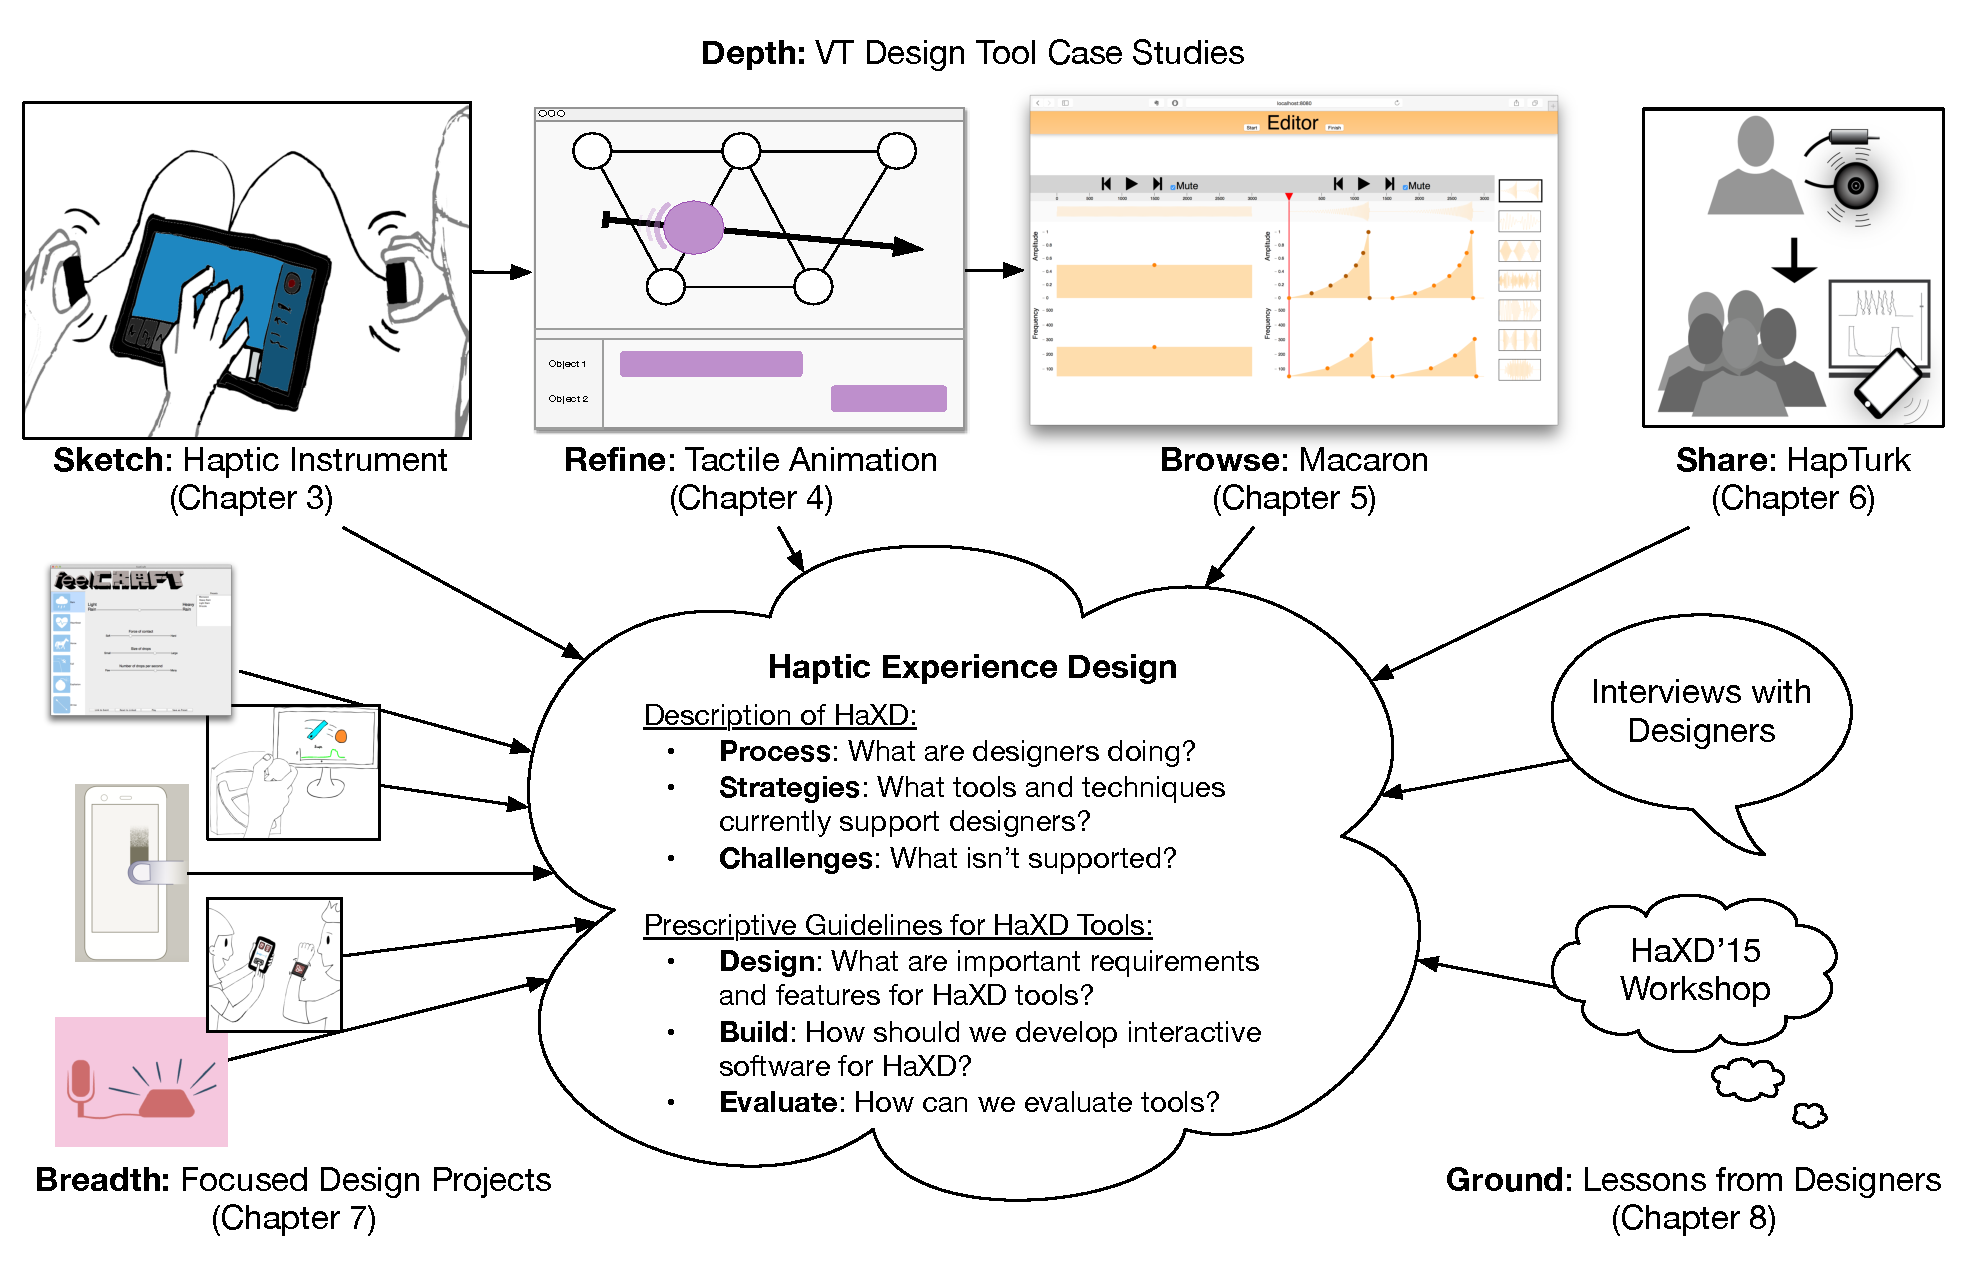
\includegraphics[width=\textwidth]{HaXDTheoryOutline-2016-08-11}
\caption{Approach overview. We investigate VT design tools (Chapters \ref{ch:hapticinstrument}-\ref{ch:macaron}) and techniques (Chapter \ref{ch:hapturk}) in-depth. These findings are synthesized with multiple, smaller focused projects (Chapter \ref{ch:applications}) and grounded data from hapticians (Chapter \ref{ch:hapticianinterviews}) into a preliminary understanding of \haxd.}
\label{fig:intro:methodologyoverview}
\end{center}
\end{figure}



\section{Approach}
%While many tools exist to support design in other modalities, there are few for haptics.
%Part of this comes from immaturity of the field and lack of market penetration of highly expressive haptic devices.
%However, there are also intrinsic challenges to designing for the sense of touch.
%I want to develop practical tools that support the HaXD process, building a body of knowledge of how to facillitate this difficult subfield of design.
We approach this problem with three strategies: vibrotactile design tool case studies for depth, several focused design projects for breadth, and data from haptic designers to ground our findings  (\autoref{fig:intro:methodologyoverview}).

\subsection{Depth: Vibrotactile design tool case studies (Chapters \ref{ch:hapticinstrument}-\ref{ch:hapturk})}
To understand design, we take a design perspective.
In each of three case studies, we design, build, and evaluate a tool or technique to support an aspect of \haxd, scoped to \emph{vibrotactile} (VT) design.
Each of these results in concrete implications for designing tools and a small window onto the larger HaXD process.
Contributions include algorithms, data structures, interaction techniques, features, analytic techniques, and working software tools that have been employed by designers.
\autoref{ch:hapticinstrument}, \autoref{ch:tactileanimation}, and \autoref{ch:macaron} outline iterative development and evaluation of VT design tools; \autoref{ch:hapturk} covers a VT design technique (proxies).

\subsection{Breadth: Focused haptic design projects (Chapter \ref{ch:applications})}
While the case studies provide an in-depth investigation into VT sensation design, results may not generalize to other devices, and provide limited investigation into application areas like education.
To generalize from VT effects, explore other aspects of haptic design, and gain personal experience as haptic experience designers, we participate in several smaller focused design projects, which lend a broader context to our findings.
\autoref{ch:applications} discusses these projects.

\subsection{Ground: Data from haptic experience designers (Chapter \ref{ch:hapticianinterviews})}
Despite the recent growth of the field, haptic designers remain relatively rare and difficult to recruit.
To complement our primarily design-based approach and ground it with haptic experience designers in the field, we draw from other data sources: a workshop held at World Haptics 2015 and interviews with haptic designers.
\autoref{ch:hapticianinterviews} discusses this characterization of \haxd, and serves as a capstone by defining \haxd and articulating a vision for how \haxd might manifest.




\section{Outline and Contributions}
This dissertation continues as follows.
First, in \autoref{ch:rw}, we present the necessary background with an overview of haptic technology and perception, the value of haptics and related applications,  design theory from non-haptic fields,  existing haptic design tools and techniques, and underlying methodology of our work.

Then, we outline each VT case study in Chapters \ref{ch:hapticinstrument}-\ref{ch:hapturk}.
In \autoref{ch:hapticinstrument}, we present findings from our first vibrotactile design tool, the haptic instrument, which supported easy exploration and informal feedback (\emph{sketching}), but identified a key problem: it did not support \emph{refining} designs.

In \autoref{ch:tactileanimation}, we present findings from our second vibrotactile design tool, Mango, which established a generalized pipeline and was able to support both \emph{sketching} and \emph{refining} for expert visual animators; it highlighted reuse as an important next step.

In \autoref{ch:macaron}, we present findings from our third vibrotactile design tool, Macaron, which implemented a \emph{browsing} interface and analytics system; we found examples played a large part of the design process, and used user logs to provide a picture of our participants' design process, including confirmation of project preparation and \emph{browsing}, initial design, \emph{sketching}, and \emph{refining}.

In \autoref{ch:hapturk}, we document findings from HapTurk, a technique for \emph{sharing} vibrotactile designs for feedback at scale: from the crowd using proxy vibrations distributed over Mechanical Turk. 

%Each chapter is presented as a direct outline of what will appear in the final dissertation, summarizing either methods and results (\autoref{ch:hapticinstrument} and \autoref{ch:hapticanimation}) or proposed methods and possible results (\autoref{ch:hapticexamples}).
We then describe focused haptic design projects in \autoref{ch:applications}, and the results from our grounded data collection in \autoref{ch:hapticianinterviews}.\
In \autoref{ch:applications}, we synthesize together findings from our side projects, showing generality by applying our understanding of haptic design explicitly in several domains and gaining practical experience designing haptic experience.

In \autoref{ch:hapticianinterviews}, we complement our design-based inquiry through interviews with professional haptic designers and a workshop run to elicit feedback from the community; this captures a description of haptic design, reinforcing our findings for important support tools, and identifies more systematic challenges.

Finally, in \autoref{ch:conclusion}, we conclude with a synthesis of our final results and directions for future research.


%
% END
%
\endinput

Any text after an \endinput is ignored.
You could put scraps here or things in progress.
